%! TEX root = ./main.tex

\lecture{5}{Week: 3}{C Pointers}

\subsubsection{Address Space}
The OS gives each process an address space, which contains the virtual memory. The virtual memory is visible only to the process. Each byte is addressable and there are $2^{64}$ bytes of memory on a $64$ bit machine. The OS maps the virtual memory to the physical memory.
When the OS loads a program, the following steps are executed:

\paragraph{Loading a program}
\begin{itemize}
    \item create an address space
    \item inspect the executable file
    \item copy regions of the file into memory space
    \item do final linking, reallocation or other preparations
\end{itemize}

\subsubsection{Stack}
The stack is allocated in frames. The current procedure's frame always lies on the top of the stack. The frame stores local variables, return types etc. On recursive calls, for each recursion a new frame is pushed to the stack

\subsubsection{C Pointers}
Pointers are variables which store memory addresses. \code{\&x} gives the virtual address where the value of variable \code{x} is stored. With \code{\%p} its value can be printed. Pointers are declared using the format \code{type *name;}. Dereferencing a pointer means accessing the memory referred by the pointer. This way we can access the value at the address or write some value to the address. Double pointers are pointers which point to a pointer. They are declared using \code{type **name;}. Double pointers are mostly used for multidimensional arrays.

The address space layout randomization is responsible that the stack bases and shared library location addresses change for each execution. This is a security feature which makes debugging tougher. But it could be disabled.

\code{NULL} is a \textit{guaranteed-to-be-invalid} memory location and has type \code{void *}. Dereferencing \code{NULL} causes a segmentation fault. \code{NULL} is useful to mark end points and invalid addresses.

A \code{*} is used to indicate that a function returns a pointer as \code{int *getPtr()}.

\subsubsection{Pointer Arithmetic}
When incrementing a pointer by $1$, the value of the pointer (address) is incremented by the size of the type of the pointer. For integer this is e.g. $4$ bytes, for double $8$ bytes, for char $1$ byte etc... These values depend on the machine and compiler. The size can be evaluated using \code{sizeof(type)} or \code{sizeof(value)}.

\subsubsection{Arrays and Pointers}
An array is a collection of homogeneous data elements stored at contiguous memory adresses. A Pointer is a variable that stores a memory address. So pointers and arrays are different, but related things. The array name is an expression and treated as a pointer to the first element of the array \code{a == \&(a[0])}. We can access the array by the \textit{pointer} $+$ some offset. The compiler rewrites \code{A[i]} to \code{*(A+i)}, hence we could theoretically access arrays like \code{i[A]}.\\
However, the array name is different from the pointer when:
\begin{enumerate}
    \item The array is an operand of \code{sizeof()}
\begin{lstlisting}
int a[10]:
assert(sizeof(a) == 10 * sizeof(int));
assert(sizeof(&a[0] == sizeof(int *));
\end{lstlisting}
    \item The array's address is taken with \code{\&}
\begin{lstlisting}
int a[10];
assert(&a == a);
\end{lstlisting}
    \item The array is string literal initializer
\begin{lstlisting}
char a[] = "Hello!";
char *b = "Hello!"; // undef. behaviour when modified
\end{lstlisting}
\end{enumerate}
In C, parameters are passed as value (since there is nothing like a reference), with the only exception of arrays and functions. They are passed by pointers. Therefore, the following three formal arguments \code{int *arr}, \code{int arr[]} and \code{int arr[10]} are equivalent.\\ 
Arrays cannot be renamed, but we change the pointer.

\subsubsection{Passed by Reference}
Since C is passed by value, we can pass a reference by passing a pointer. However, this pointer is again passed by value and therefore can be modified in the scope of the functions.

\subsubsection{Examples}
Here some pointer declaration examples:

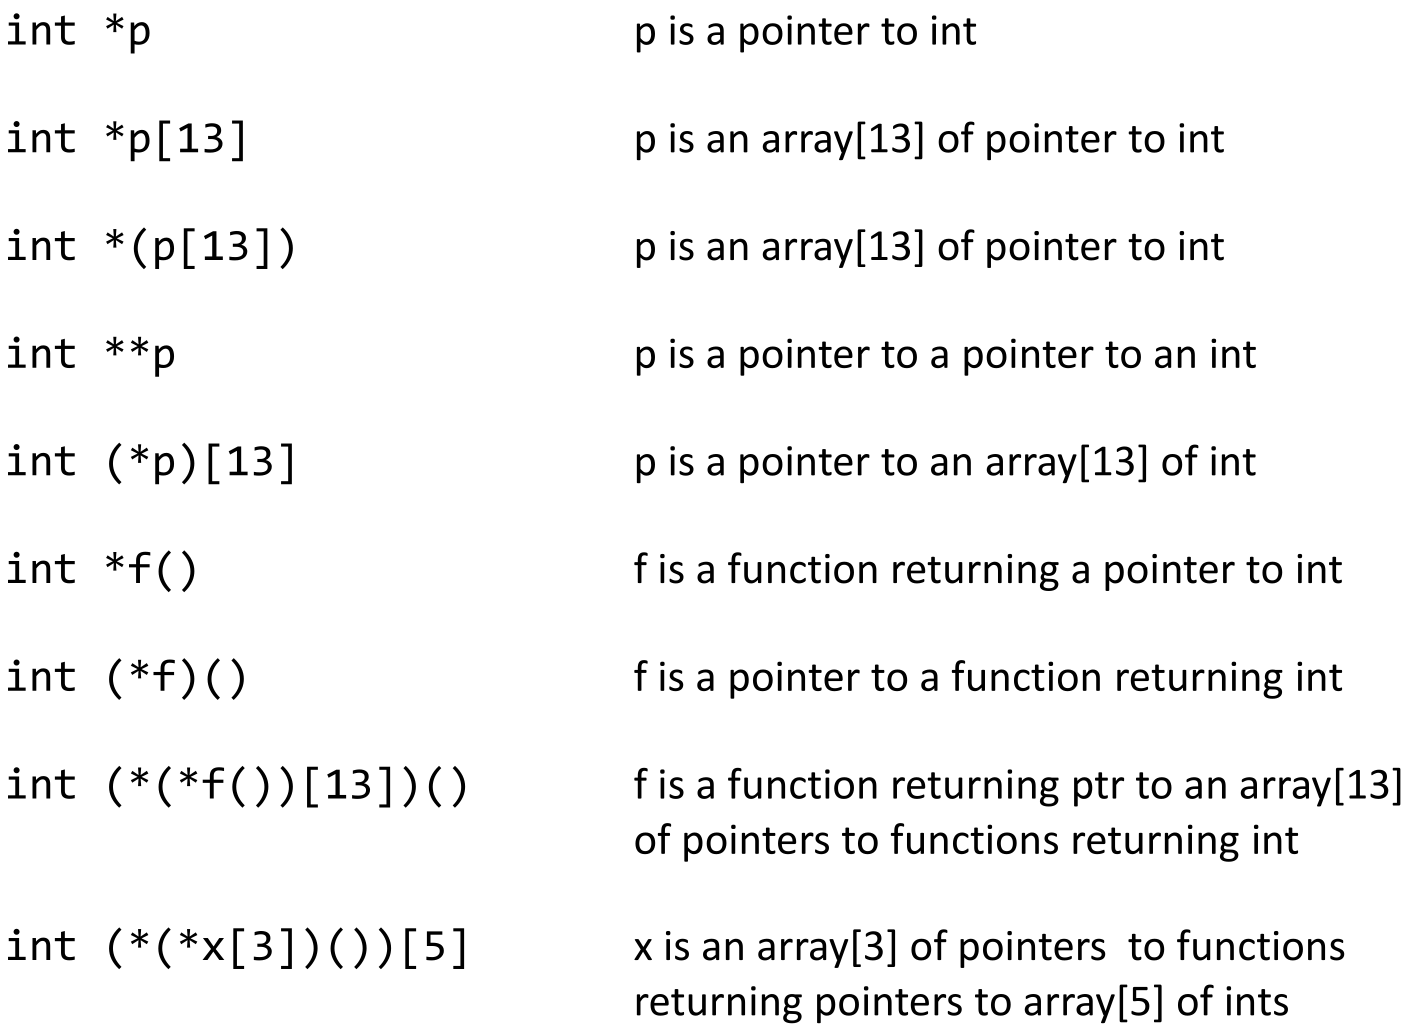
\includegraphics[width=0.8\textwidth]{05_pointerDeclarationEx.png}
